\documentclass[10pt,letterpaper]{article}
%\usepackage{times}
\usepackage[margin=1in,hmargin=1in]{geometry}
\usepackage{amsmath}
\usepackage{tikz,url}
\usepackage{amssymb}
\usepackage{fancyhdr}
\usetikzlibrary{matrix}
\usepackage{listings}
\usepackage{tabularx}
\usepackage{xcolor}
\usepackage{graphicx}
\usepackage{graphics}
\usepackage{titling}
\pagestyle{fancy}
\usepackage{float}
\usepackage{fancyvrb}
\usepackage{verbatim}
\usepackage{enumitem}
\usepackage{alltt}
\usepackage{pdfpages}
\usepackage{multicol}
%\restylefloat{table}

\fancyhead[LO]{STAT W4201 Advanced Data Analysis}
\fancyhead[RO]{HW 9}
\fancyhead[LE]{STAT W4201 Advanced Data Analysis}
\fancyhead[RE]{HW 9}
\title{\textbf {Homework 9}}
\author{{Qianbo Wang}\\{uni: qw2180}}
\date{}
\setlength{\droptitle}{-5em}
\setlength{\parindent}{0pt}
\makeatletter
\newcommand{\rmnum}[1]{\romannumeral #1}
\newcommand{\Rmnum}[1]{\expandafter\@slowromancap\romannumeral #1@}
\makeatother

\lstset{
language=R,
tabsize=4, 
%frame=shadowbox, 
commentstyle=\color{red!50!green!50!blue!50},
%rulesepcolor=\color{red!20!green!20!blue!20},
keywordstyle=\color{blue!90},
showstringspaces=false,
stringstyle=\ttfamily, 
keepspaces=true, 
breakindent=22pt, 
numbers=none,
stepnumber=1,
numberstyle=\tiny, 
numberstyle={\color[RGB]{0,192,192}\tiny} ,
numbersep=5pt,  
basicstyle=\footnotesize, 
showspaces=false, 
flexiblecolumns=true, 
comment=[l]{\#},
texcl=true,
escapeinside={\$$}{\^^M},
escapechar=\&
breaklines=true, 
breakautoindent=true,
breakindent=4em, 
aboveskip=1em, 
tabsize=2,
showstringspaces=false, 
backgroundcolor=\color[RGB]{244,244,244},   
fontadjust,
captionpos=t,
framextopmargin=2pt,framexbottommargin=2pt,abovecaptionskip=-3pt,belowcaptionskip=3pt,
extendedchars=false,columns=flexible
}

\RecustomVerbatimCommand{\VerbatimInput}{VerbatimInput}{fontsize=\footnotesize}
\begin{document}
\maketitle
\thispagestyle{fancy}
\vspace{-2em}
\textbf{Consider the colon data in the R package "survival". It gives adjuvant chemotherapy data for colon cancer. Levamisole is a low-toxicity compound previously used to treat worm infestations in animals; 5-FU is a moderately toxic (as these things go) chemotherapy agent. There are two records per person, one for recurrence (etype=1) and one for death (etype=2). Other important variables include: 
\begin{enumerate}[leftmargin=0cm,itemindent=.5cm,labelwidth=\itemindent,labelsep=0cm,align=left]
\item[\textbullet] rx: Treatment: Obs(ervation), Lev(amisole), Lev(amisole)+5-FU 
\item[\textbullet] sex: 1=male 
\item[\textbullet] age: in years 
\item[\textbullet] time: days until event or censoring 
\item[\textbullet] status: censoring status
\end{enumerate}
For the following, consider survival to be “Days until Death”, i.e., etype=2.}
\section*{Problem 1}
\textbf{Using the Kaplan-Meier method, estimate the survival curve for each treatment group: Lev(amisole) and Lev(amisole)+5-FU.}\\

Using Kaplan-Meier method, fit the survival estimator, the estimated survival curve is as follows:
\begin{center}
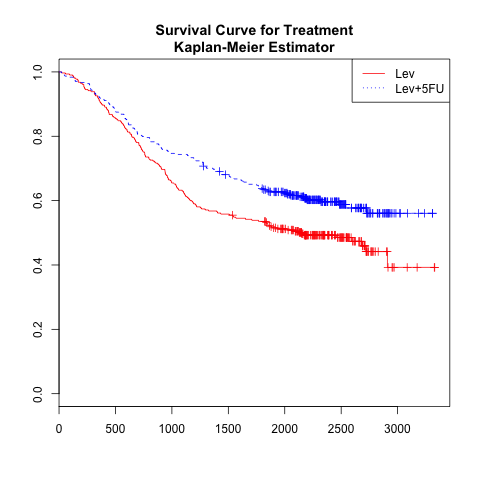
\includegraphics[scale=0.5]{meiercurve}
\end{center}
\section*{Problem 2}
\textbf{Estimate the median survival time for each of the two treatment groups, using the estimated survival curves.}\\

Using Kaplan-Meier survival curve, the result is as follows:
\begin{center}
\small{Kaplan-Meier Estimated Curve}
\VerbatimInput{meier.txt}
\end{center}
So the estimated median is:
\begin{table}[H]
\caption{Estimated Median for two treatment groups}
\centering
\begin{tabular*}{0.4\linewidth}{@{\extracolsep{\fill}}ccc}
\hline
Treatment & Lev & Lev+5FU\\
\hline
 Median & 2152 & NA \\
\hline
\end{tabular*}
\end{table}
The median is calculated as the smallest survival time for which the survivor function is less than or equal to 0.5. 
\begin{enumerate}[leftmargin=0cm,itemindent=.5cm,labelwidth=\itemindent,labelsep=0cm,align=left]
\item[\textbullet] For treatment Lev, the estimated median is 2152.
\item[\textbullet] For treatment Lev+5FU, since it never gets to the point where $s(t) \leq 0.5$, then the median for treatment Lev+5FU is NA.
\end{enumerate}
\section*{Problem 3}
\textbf{Using the log-rank test, determine whether there is a difference in survival between the two groups.}\\

Using Log-rank test, the null hypothesis and alternative hypothesis are:
\begin{equation*}
\begin{split}
\text{H\textsubscript{0}:} & \ \text{there is no difference between the two treatment of survival curves} \\
\text{H\textsubscript{1}:} & \ \text{there is difference between the two treatment of survival curves}\\
\end{split}
\end{equation*}
the result is as follows:
\begin{center}
\small{Log-rank Test Result}
\VerbatimInput{logrank.txt}
\end{center}
Since the p-value of log-rank test is 0.00417, then we should reject the null hypothesis, i.e., concluding that there is a difference in survival between the two groups.
\section*{Problem 4}
\textbf{Using a Cox proportional hazards model, estimate the hazard ratio for Levamisole relative to 5-FU, adjusting for Age and Sex.}\\

Using Cox proportional hazards model and adjusting for Age and Sex, the result is as follows:
\begin{center}
\small{Cox proportional hazards model adjusting for age and sex Result}
\VerbatimInput{cox.txt}
\end{center}
Since we want to get the hazard ratio for Levamisole relative to 5-FU, then we simply set the Lev+5FU as the baseline.\\

Since from the result we can see, the hazard ratio for the second group relative to the first group, that is, rxLev relative to rxLev+5FU with adjusting for age and sex is 1.4115.
\section*{Problem 5}
\textbf{Give a 95\% confidence interval for the hazard ratio in 4.}\\

From the result above, we can see that the 95\% confidence interval for hazard ratio in Problem 4 is: \[[1.1155 , 1.786]\] 

\newpage
\textbf{R Code:}
\begin{lstlisting}
rm(list = ls())
library(survival)
data("colon")

#Meier Estimator for treatment Lev, Lev+5FU
survival_colon <- subset(colon,etype==2 & rx %in% c("Lev","Lev+5FU"))
fit_trt<- survfit(formula = Surv(time, status) ~ rx, data = survival_colon, type = "kaplan-meier")
sink('/Users/raymond/Drive/STAT W4201/HW9/meiersum.txt')
summary(fit_trt)
sink()

#Plot the survival curve
png(filename = "/Users/raymond/Drive/STAT W4201/HW9/meiercurve.png")
plot(fit_trt,lty = c(1,2),col = c("red","blue"))
title(main="Survival Curve for Treatment")
title(main="Kaplan-Meier Estimator",line=0.5)
legend("topright",c("Lev","Lev+5FU"),col=c("red","blue"),lty=c(1,3))
dev.off()

#Estimate the median
sink('/Users/raymond/Drive/STAT W4201/HW9/meier.txt')
fit_trt
sink()

#Log-rank test for difference
log_rank<-survdiff(Surv(time, status) ~ rx, data=survival_colon)

sink('/Users/raymond/Drive/STAT W4201/HW9/logrank.txt')
log_rank
sink()

#Cox proportional hazards model
survival_colon$rx_d<-as.numeric(survival_colon$rx=="Lev")
cox<-coxph(Surv(time,status)~rx_d+age+sex,data=survival_colon)
sink('/Users/raymond/Drive/STAT W4201/HW9/cox.txt')
summary(cox)
sink()

\end{lstlisting}
\end{document}